%!TEX root = ../Physik I.tex

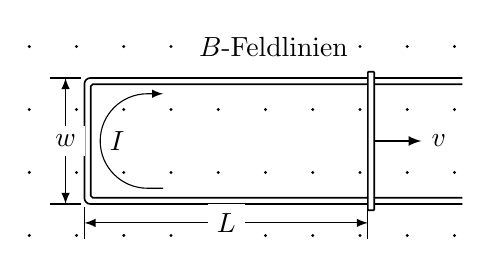
\begin{tikzpicture}[>=latex,scale=.4]
	\begin{scope}
		\foreach \x in {-1.75,-.25,...,12}
			\foreach \y in {-3,-1,...,3}
				\fill (\x,\y) circle (1.5pt)
			;
		;
		\draw (6,3) node[fill=white]{$B$-Feldlinien};
	\end{scope}
	\begin{scope}[semithick]
		\draw[rounded corners=.075cm]
			(12,2) -- (0,2) -- (0,-2) -- (12,-2)
		;
		\draw[rounded corners=.025cm]
			(12,1.8) -- (.2,1.8) -- (.2,-1.8) -- (12,-1.8)
		;
		\filldraw[fill=white,rounded corners=.01cm]
			(9,2.2) -- (9.2,2.2) -- (9.2,-2.2) -- (9,-2.2) -- cycle
		;
		\draw[->]
			(9.2,0) -- (10.7,0) node[right]{$v$}
		;
	\end{scope}
	\begin{scope}[xshift=-.1cm]
		\draw
			(-1,-2) -- (0,-2)
			(-1,2) -- (0,2)
		;
		\draw[<->] (-.5,-2) -- (-.5,2) node[pos=.5,fill=white]{$w$};
	\end{scope}
	\begin{scope}[yshift=-.1cm]
		\draw
			(0,-2) -- (0,-3)
			(9,-2) -- (9,-3)
		;
		\draw[<->] (0,-2.5) -- (9,-2.5) node[pos=.5,fill=white]{$L$};
	\end{scope}
	\begin{scope}
		\draw[->,rounded corners=.6cm]
			(2.5,-1.5) -- (.5,-1.5) -- (.5,1.5) node[pos=.5,right]{$I$} -- (2.5,1.5)
		;
	\end{scope}
\end{tikzpicture}